\documentclass[english,notblind]{sbc20}

\usepackage{verbatim}  % support for unformatted text, almost mandatory
\usepackage{graphicx}  % support for figures etc., almost mandatory
\usepackage{array}     % extra table features, almost mandatory
%\usepackage{pbalance}  % equal heights in last page columns (demands additional LaTeX passes)
%\usepackage{mathtools} % extra visual tweaks/features for math, read the docs

% Table improvements
\usepackage{booktabs}  % better table aesthetics, recommended, read the docs
\usepackage{multirow}  % table cells that span over multiple rows
\usepackage{makecell}  % better table headings / cells with linebreaks inside
\usepackage{dcolumn}   % align numeric columns on the decimal separator (siunitx also offers this)
%\usepackage{longtable} % multi-page tables
%\usepackage{threeparttable} % tables with "footnotes"
%\usepackage{colortbl}  % colored table cells
%\usepackage{csvsimple} % load a csv file and format as table

% Extra features for floats
%\usepackage{rotating}   % \sidewaystable, \sidewaysfigure, and other rotation commands
%\usepackage[above,below]{placeins} % manually control float placement, read the docs
%\usepackage{subcaption} % subfigures (side by side) with subcaptions (pkg subfigure is deprecated)
%\usepackage{adjustbox}  % resize, clip etc. for any material, not only floats

% Source code syntax highlighting
%\usepackage{listings} % good and simple
%\usepackage{minted}   % excellent, but depends on pygments (python, free software)

%\usepackage{siunitx} % Numbers: units, scientific notation, better presentation for large numbers

%\usepackage{pdfcomment} % useful in the writing/reviewing phase


\addbibresource{bibliografia.bib}

\metadata
  {
    pubname={Escola Regional de Redes de Computadores},
    pubacron={ERRC},
    idjems={XXX},
    copyrightyear=2024,
    category={Full Paper},
    bibstyle=sbc20,
  }
  
\title
  {
    mainlanguagetitle={RouteBastion: Architecting a VRP API Broker},
  }

\shortauthor{Vieira et al. 2024}
\shorttitle{RouteBastion: Architecturing a VRP API Broker}

\author
  {
    email=pietrovieira.aluno@unipampa.edu.br,
    orcid=0009-0004-0602-6567,
    institutionID=UNIPAMPA,
    country=Brasil,
    firstName=Pietro,
    lastName=Vieira 
  }
  
  \author
  {
    email=dalmazo@furg.br,
    orcid=0000-0002-6996-7602,
    institutionID=FURG,
    country=Brasil,
    firstName=Bruno,
    lastName=Dalmazo 
  }

\author
  {
    email=rodrigomansilha@unipampa.edu.br,
    orcid=0000-0002-2083-653X,
    institutionID=UNIPAMPA,
    country=Brasil,
    firstName=Rodrigo,
    lastName=Mansilha 
  }
  
\institution{UNIPAMPA}{Universidade Federal do Pampa}
\institution{FURG}{Universidade Federal do Rio Grande}


\extraAffiliationsLast{Pietro Vieira is a student at the Graduate Program in Software Engineering at UNIPAMPA. Bruno Dalmazo is a assistant professor at FURG. Rodrigo Mansilha is the coordinator of the Graduate Program in Software Engineering and a professor at UNIPAMPA.}

\abstract
  {
        The Vehicle Routing Problem (VRP) presents significant challenges to both academia and industry. Optimizing vehicle routes while balancing multiple real-life constraints, such as time windows, vehicle capacity, and fuel consumption, demands not only great computational power but also advanced problem-solving techniques. In response, major tech companies have developed cloud-based APIs to tackle this issue, offering powerful solutions that vary in terms of cost, capabilities, and performance. With multiple APIs available, selecting the right one for a given context—whether optimizing for cost, input size, or specific constraints—becomes a complex decision. In this paper, we present the architecture of RouteBastion, a Software as a Service (SaaS) platform designed to unify and simplify the use of VRP-related APIs. RouteBastion leverages a modular, scalable microservice architecture built with [insert technologies here], allowing users to evaluate and select the most appropriate API based on their needs. By providing seamless integration, dynamic API selection, and support for real-time decision-making, RouteBastion serves as an intelligent middleware that enhances both the flexibility and accessibility of vehicle route optimization. This paper will delve into the system architecture, the decision-making algorithms employed, and the performance considerations that ensure RouteBastion can adapt to evolving industrial requirements.
  }

\keywords{Vehicle Routing Problem \sep VRP \sep Software Architecture \sep Software as a Service}

\palavraschave{Problema de Roteamento de Veículos \sep PRV \sep Arquitetura de Software \sep Software como Serviço}


\contributeinfo{ }

\acknowledgements{ }

\funding{ }

\datainfo{ }

\furtherinfo{ }

\SBCprintbibliography

\begin{document}

\maketitle

\section{Introduction}
\label{sec:intro}

The Vehicle Routing Problem (VRP) is a classic optimization challenge that has garnered attention from both academia and industry due to its significant real-world applications. Efficiently managing a fleet of vehicles to service multiple locations under various constraints—such as delivery time windows, vehicle capacities, and route costs—has the potential to greatly enhance logistics, reduce fuel consumption, and improve customer satisfaction. However, solving the VRP is complex, often classified as NP-hard, meaning that computational demands increase exponentially as the problem size grows.

To address this complexity, many large-scale technology companies have developed powerful cloud-based APIs aimed at providing route optimization as a service. These APIs often combine sophisticated algorithms with scalable cloud resources to tackle the VRP across diverse industries, from e-commerce to transportation. Solutions from companies like Google, Microsoft, and others offer varying degrees of optimization based on specific parameters such as cost-efficiency, speed, or the ability to handle large datasets. However, given the diversity of API offerings, companies often face a difficult decision: which service best meets their needs in terms of functionality, performance, and cost-effectiveness?

In this context, selecting the most appropriate API is not a trivial task. The need for flexibility and customization across varying use cases—whether for optimizing cost, increasing input size, or adapting to specific business constraints—complicates the decision further. Enterprises may find themselves limited by the features or pricing structures of a single API, or they may need to constantly switch between services to best suit different routing scenarios.

This paper introduces RouteBastion, a Software as a Service (SaaS) solution designed to solve this problem by unifying multiple Vehicle Routing Problem APIs into a single platform. RouteBastion abstracts the complexity of comparing and integrating different APIs by providing a seamless, centralized service where users can dynamically select the most suitable API for their needs. The platform’s architecture is built on principles of modularity and scalability, ensuring that it can accommodate the constantly evolving landscape of route optimization services. This SaaS platform will offer more than just API aggregation; it will incorporate intelligent decision-making mechanisms, allowing users to optimize route planning not only based on individual API strengths but also on real-time operational requirements, such as route complexity, input size, or pricing considerations.

The remainder of this paper will explore the architectural design of RouteBastion, discussing its structure and the performance considerations that will make it a robust solution for industrial-grade VRP optimization.

\section{Theoretical framework}
\label{sec:theoretical_framework}

This section outlines the foundational concepts and technologies that underpin the design and implementation of RouteBastion. Specifically, it covers the C4 model for software architecture, the Go programming language, the REST architectural pattern and the gRPC open-source RPC framework.

\subsection{C4 Model for Software Architecture}
\label{subsec:c4_model_for_software_architecture}
The C4 model \cite{c4model} is a widely used approach for visualizing and documenting software architecture at multiple levels of abstraction. Introduced by Simon Brown, C4 stands for Context, Container, Component, and Code, which are the four levels of diagrams used to describe software systems. The model helps architects and developers break down complex systems into understandable parts by starting with a high-level overview (context) and progressively drilling down into more detailed views (containers, components, and code). This hierarchical structure enables clear communication among stakeholders, making it easier to reason about the design and behavior of the system. In RouteBastion, the C4 model is used to depict both the overall system interaction (context) and the internal architecture of the broker (container), offering a clear understanding of how external software systems, cloud providers, and internal components interact.

\subsection{Go Programming Language (Golang)}
\label{subsec:go_programming_language}
Go \cite{gopl}, often referred to as Golang, is an open-source programming language designed by Google with a focus on simplicity, performance, and scalability. Its statically typed nature, coupled with a rich set of built-in features like concurrency via goroutines, makes it highly suitable for building distributed and scalable systems. Go’s efficient memory management and ability to handle multiple tasks concurrently make it an excellent choice for backend services that need to manage numerous simultaneous connections, such as API gateways. In RouteBastion, Go will be used to implement the Broker API, providing the scalability and performance required to handle large volumes of route optimization requests from external systems while ensuring minimal latency in selecting the appropriate cloud provider for each request.

\subsection{REST Architectural Pattern}
\label{subsec:rest}
The Representational State Transfer (REST) is a widely adopted architectural pattern for designing networked applications. It relies on stateless communication and well-defined methods (GET, POST, PUT, DELETE) to facilitate interactions between clients and servers. RESTful APIs are lightweight, making them an ideal choice for web services that need to handle a large number of requests efficiently. RouteBastion will leverage the REST pattern to expose its Broker API, enabling external systems to interact with it through simple HTTP requests. By following REST principles, RouteBastion will ensure a decoupled and flexible system where each request is self-contained, allowing for easier scalability, load balancing, and integration with different systems.

\subsection{gRPC}
\label{subsec:grpc}
gRPC (Google Remote Procedure Call) \cite{grpc} is a high-performance, open-source RPC framework designed for efficient communication between distributed systems. It uses Protocol Buffers (Protobuf) for serializing structured data, which reduces payload sizes and improves communication speed compared to traditional REST APIs, which often rely on JSON. One of gRPC's core advantages is its ability to support bi-directional streaming, allowing both clients and servers to continuously exchange data over a single connection, making it ideal for real-time communication in highly responsive systems.

In the context of RouteBastion, gRPC offers a more efficient communication layer for internal service-to-service interactions, particularly between the Broker API and cloud providers. By leveraging gRPC's compact message format and fast processing capabilities, RouteBastion can handle larger optimization workloads with lower latency, providing faster responses and better performance for route optimization queries. While REST is a practical choice for external communication, gRPC's efficiency makes it a strong candidate for optimizing internal operations, especially when dealing with high volumes of route data and cloud provider requests. It's important to note that RouteBastion will expose not only a REST API but will also expose a gRPC protocol to client systems, allowing them to take advantage of the great capabilities of gRPC too.

These four foundational elements — the C4 model, Go programming language, REST architecture and gRPC — provide the basis for the design and operational efficiency of RouteBastion. Each plays a crucial role in ensuring that the system is well-architected, scalable, and efficient.

\section{System Overview}
\label{sec:system_overview}
RouteBastion is designed as an API gateway, enabling external systems to leverage various cloud-based Vehicle Routing Problem (VRP) optimization APIs. The platform abstracts the complexity of interacting with multiple third-party VRP optimization providers, such as Google Cloud and Azure, allowing external software systems to request route optimizations without being tied to a specific provider. The core architecture of RouteBastion revolves around the RouteBastion Broker, which facilitates communication between external client systems and cloud API providers, offering dynamic API selection and optimization scheduling.

\subsection{System Context}
\label{subsec:system_context}
In the system context diagram (\ref{fig:system}), RouteBastion interacts with two main entities:

\begin{figure}
  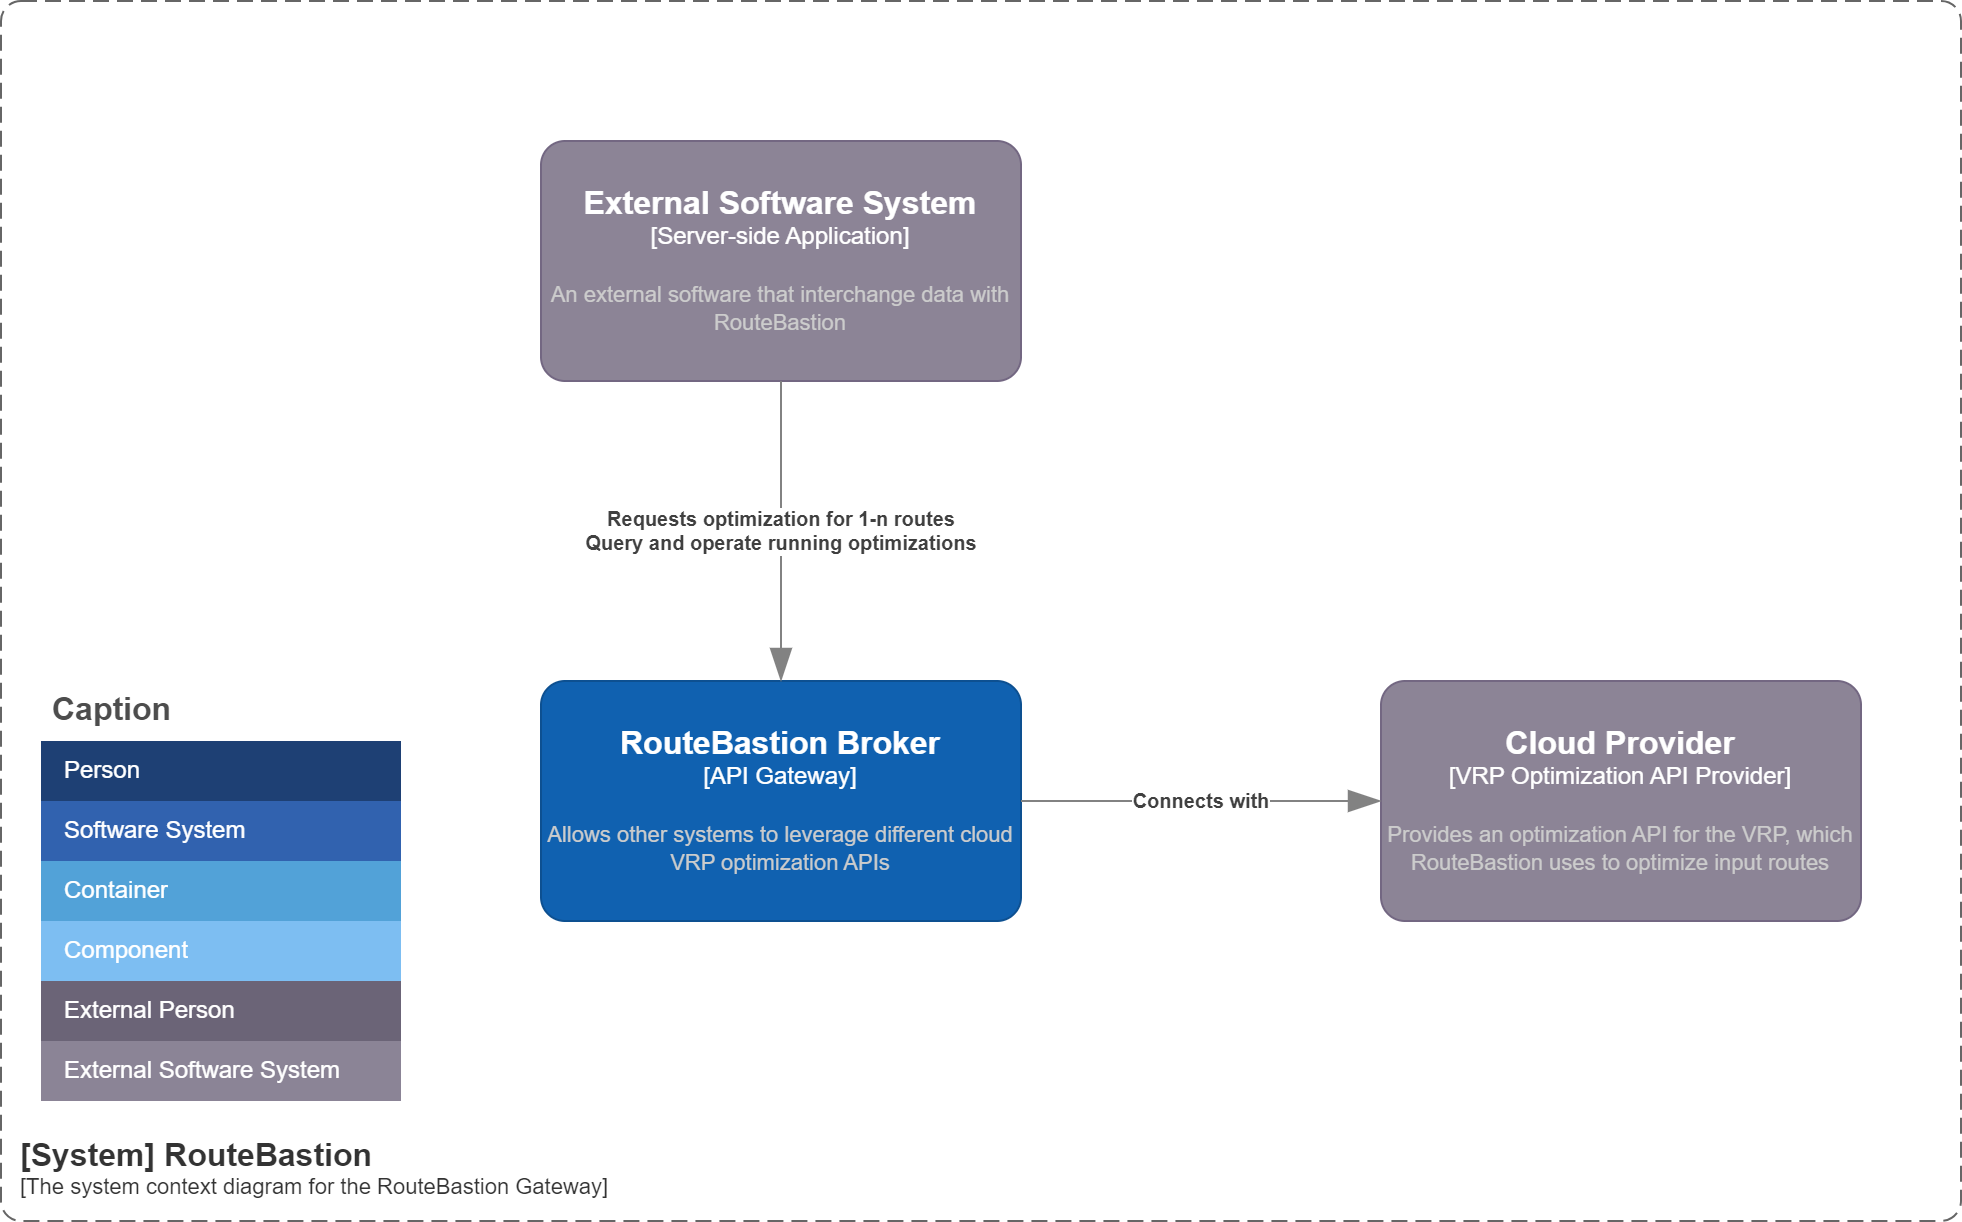
\includegraphics[width=\columnwidth]{figures/c4_diagrams/System.png}
  \caption{System Diagram\label{fig:system}}
\end{figure}

\begin{itemize}
  \item External Software System: This represents any server-side application that interacts with RouteBastion to request route optimizations or query the status of ongoing optimizations. The external system relies on RouteBastion to route these requests to the most appropriate cloud provider based on dynamic factors like cost and performance.

  \item Cloud Provider: These are VRP optimization API providers such as Google Cloud and Azure, which provide the computational resources and algorithms to solve the Vehicle Routing Problem. RouteBastion connects with these providers, leveraging their APIs to perform route optimizations for the external software systems.
\end{itemize}

At the heart of this architecture is the RouteBastion Broker, which serves as the API gateway and manages the routing of optimization requests to the cloud providers.

\subsection{Container Architecture}
\label{subsec:container_architecture}
The container diagram (\ref{fig:container}) delves deeper into the internal components of the RouteBastion Broker system, highlighting the service itself and databases that power the platform. The key components of the architecture include:

\begin{figure}
  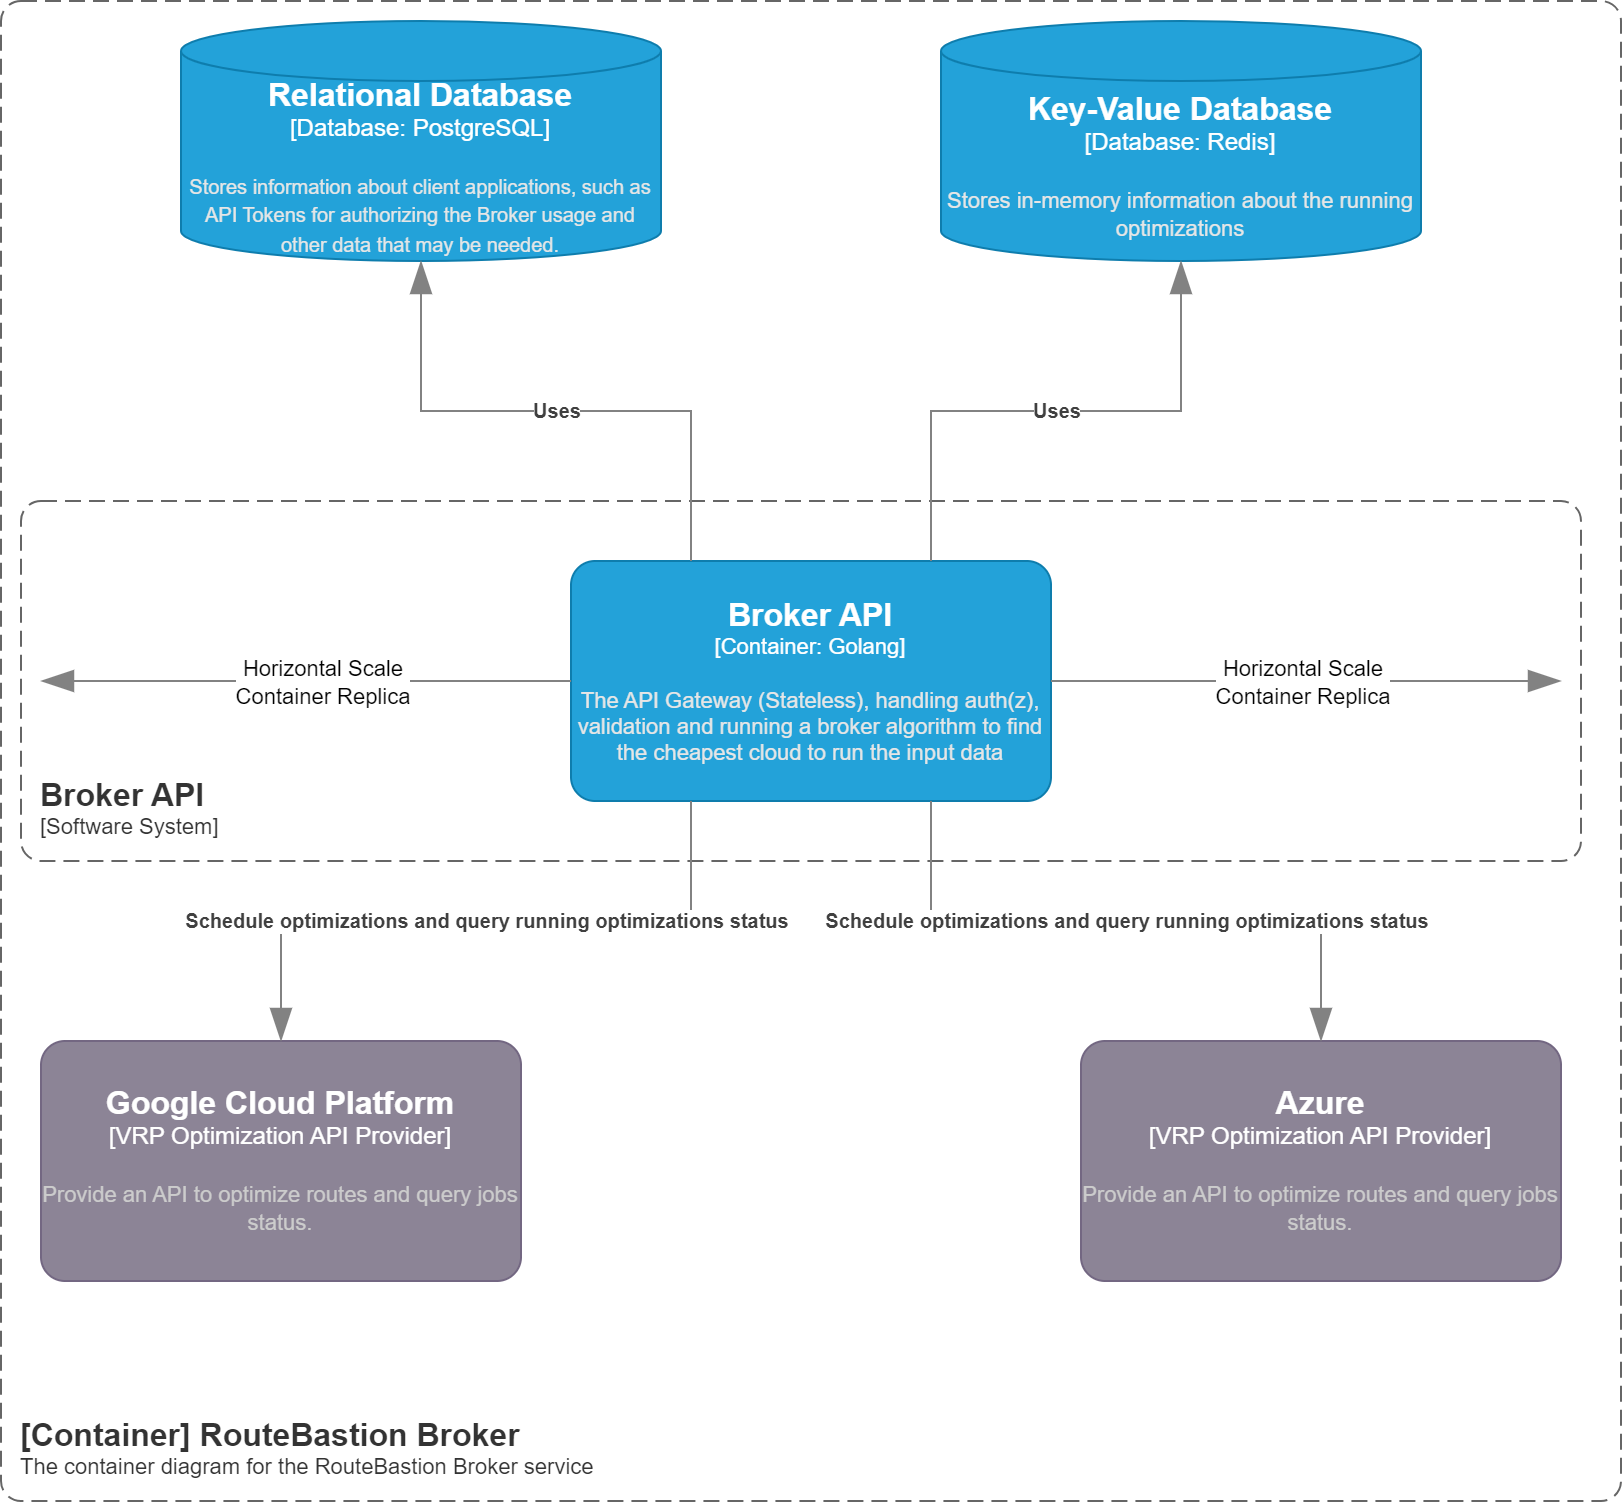
\includegraphics[width=\columnwidth]{figures/c4_diagrams/Container.png}
  \caption{Container Diagram\label{fig:container}}
\end{figure}

\begin{itemize}
  \item Broker API: The Broker API is the main container, implemented using Golang, which acts as a stateless API gateway. Its responsibilities include:
        \begin{itemize}
          \item Handling authentication and authorization for incoming requests from external systems.
          \item Validating requests before passing them to the appropriate cloud provider.
          \item Running a broker algorithm that dynamically selects the most cost-efficient cloud provider for each optimization task based on predefined criteria (e.g., input size, cost).
        \end{itemize}

  \item Relational Database (PostgreSQL): This component stores persistent data, such as information about client applications (e.g., API tokens for authorization), usage statistics, and other metadata required for managing the system's operations.

  \item Key-Value Database (Redis): Redis is used to store in-memory data about running optimizations. It allows the system to quickly access real-time information, such as the current status of optimizations, which is essential for monitoring and querying the ongoing optimization processes.

  \item Cloud Providers: These are external services such as Google Cloud and Azure, which provide the actual optimization algorithms and computational power to solve the VRP. The Broker API schedules optimization jobs with these cloud providers and retrieves job statuses, allowing it to present the results back to the external software systems.
\end{itemize}

The Broker API is horizontally scalable, meaning that additional replicas can be deployed to handle increased loads, ensuring the system can process high volumes of route optimization requests simultaneously.

\section{Architectural Highlights}
\label{sec:architectural_highlights}
The architecture of RouteBastion is designed for modularity and scalability, utilizing containerized services to enable horizontal scaling and efficiently handle high traffic from external systems. The stateless Broker API ensures seamless scaling by offloading state management to Redis and PostgreSQL, which store real-time data and persistent information, respectively. A key feature of the architecture is its intelligent API selection, where the broker algorithm dynamically chooses the most cost-effective or suitable cloud provider for each optimization request, optimizing for both cost and performance. The use of Redis for in-memory data storage ensures low-latency access to ongoing optimization statuses, enabling real-time performance and rapid response to status queries. Overall, this architecture provides a robust, flexible, and efficient foundation for managing complex route optimizations across multiple cloud providers.

\section{Conclusion}
In conclusion, the architecture of RouteBastion is designed to provide an efficient and scalable solution for optimizing vehicle routing through the integration of various cloud-based APIs. By leveraging the C4 model for clear architectural visualization, the Go programming language for high-performance service execution, and REST for flexible external communication, RouteBastion ensures that users can seamlessly choose and interact with the most cost-effective and capable cloud provider for their routing needs. Additionally, the potential use of gRPC for internal communication further enhances system performance, allowing the platform to handle large-scale route optimization tasks with minimal latency. This thoughtful combination of technologies positions RouteBastion as a robust and future-proof SaaS offering in the vehicle routing domain.

% \begin{itemize}
%   \item @Book: \cite{Knuth:96}.

%   \item @Article (em periódico): \cite{floats2014}.

%   \item @InProceedings (ou @Conference): \cite{alves03:simi}.

%   \item @InCollection (capítulo de livro ou coletânea): \cite{bobaoglu93:concepts}.

%   \item @Misc: \cite{gridftp}.

%   \item @article (para referência a página web): \cite{alon09:how}.

% \end{itemize}


\end{document}
